Deep Neural Networks (DNNs) consists of connected layers of different types. These types of layers will be discussed in this section

\subsection{Fully Connected layer}

A Fully Connected (FC) layer is a layer where every neuron from the previous layer is connected to every neuron in the next layer (See Figure 1). It is the basic layer in most of Deep Learning Systems, however due to the number of operations it has a big complexity (matrix multiplication is around $O(n^3)$  in big O notation). The face images used in this study were images of size $224 \times 224$ with 3 RGB channels. If in the first hidden layer we would have 1000 nodes it would be $224 \times 224 \times 1000 = 50176000$ parameters to optimize (it is only the first layer). For this reason, we must somehow reduce the number of parameters, for example by using convolution layers. 

\subsection{Convolution layer}

Convolution Layer is an idea based on edge detection. Edge detection was one of early techniques used to solve computer vision problems, as the name suggest it allows us to detect edges in a given image (See Figure 3). The Edge detection  algorithm  is  performed using a matrix called a mask and an operation called convolution. It takes matrix of size m (size of a mask) from input image, multiply it element-wise by values in mask, sums all values and as a result returns edges detected in input image (See Figure 2). The general expression of a convolution is: 
\begin{equation}
g(x, y)=(\omega * f)(x, y)=\sum_{s=-a}^{a} \sum_{t=-b}^{b} \omega(s, t) f(x-s, y-t)
\end{equation}

Where $g(x,y)$ is the filtered image, $f(x,y)$ is the original image, $\omega$ is the filter kernel. Every element of the filter kernel is considered by $-a \leqslant s \leqslant a$ and $-b \leqslant t \leqslant b$ \footnote{Equation from Wikipedia \url{https://en.wikipedia.org/wiki/Kernel_(image_processing)}}
\newline

Using hand-engineered filters values we can detect horizontal or vertical edges (See Figure 4) but what if we want to detect some more sophisticated features like cat edges (See Figure 5)? This is where deep learning comes in: Instead of using hand-engineered filter values we can use a Gradient Descent Algorithm to find the right values for mask matrix.


What is interesting at this point is the fact that regardless of the image size, we have same number of parameters to train. No matter if our image is $20 \times 20$ pixels or $1000 \times 1000$ we need to train the same number of parameters - the number of values in filter mask. It is one of main reasons why CNNs are so popular in real life computer vision problems.

The role of convolution layer is to extract crucial information (edges) from image by using custom filter masks. The side benefit of detecting edges can be reduction of image size (it is not always the case, it depends on used padding see Sec. 3.5 Padding). Outcome of Convolution Layer (the one consisting crucial information about edges) can be then propagated to Fully Connected Layers to perform classification.


   \begin{figure}[!ht]
  \centering
  \framebox{\parbox{5.5in}{$
    \begin{bmatrix}
        0 & 0 & 0 & 10 & 10 & 10\\
        0 & 0 & 0 & 10 & 10 & 10\\
        0 & 0 & 0 & 10 & 10 & 10\\
        0 & 0 & 0 & 10 & 10 & 10\\
        0 & 0 & 0 & 10 & 10 & 10\\
        0 & 0 & 0 & 10 & 10 & 10\\
    \end{bmatrix}_{img} * \begin{bmatrix}
        -1 & 0 & 1\\
        -1 & 0 & 1\\
        -1 & 0 & 1\\
    \end{bmatrix}_{mask} =
    \begin{bmatrix}
        0 & 30 & 30 & 0\\
        0 & 30 & 30 & 0\\
        0 & 30 & 30 & 0\\
    \end{bmatrix}_{detected \: edge}
    $
    }}
  %\includegraphics[scale=1.0]{figurefile}
  \caption{Example convolution operation}
  \label{figurelabel}
\end{figure}    



\begin{figure}[!ht]
  \centering
  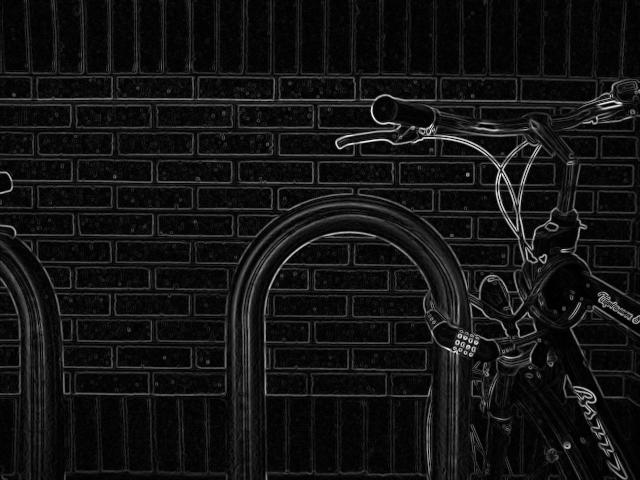
\includegraphics[scale=0.35]{Images/bikes-gray-sobel.jpg}
  \caption{Detected edges after applying Sobel filter\protect\footnotemark}
  \label{figurelabel}
\end{figure}

\footnotetext{Cat edges from \url{http://mcogswell.io/blog/why_cat_2/}}


\begin{figure}[!ht]
  \centering{
  \framebox{\parbox{4in}{
  $\begin{bmatrix}
-1 & 0 & 1\\
-2 & 0 & 2\\
-1 & 0 & 1\\
\end{bmatrix}_{0} $       $\begin{bmatrix} 
0 & 1 & 2\\
-1 & 0 & 1\\
-2 & -1 & 0\\
\end{bmatrix}_{45} $  $\begin{bmatrix}
1 & 2 & 1\\
0 & 0 & 0\\
-1 & -2 & 1\\
\end{bmatrix}_{90} $ 
}}}
  
  \caption{Example edge detection Sobel filter for angles: \ang{0}, \ang{45} and \ang{90}}
  \label{figurelabel}
\end{figure}  




\begin{figure}
\centering
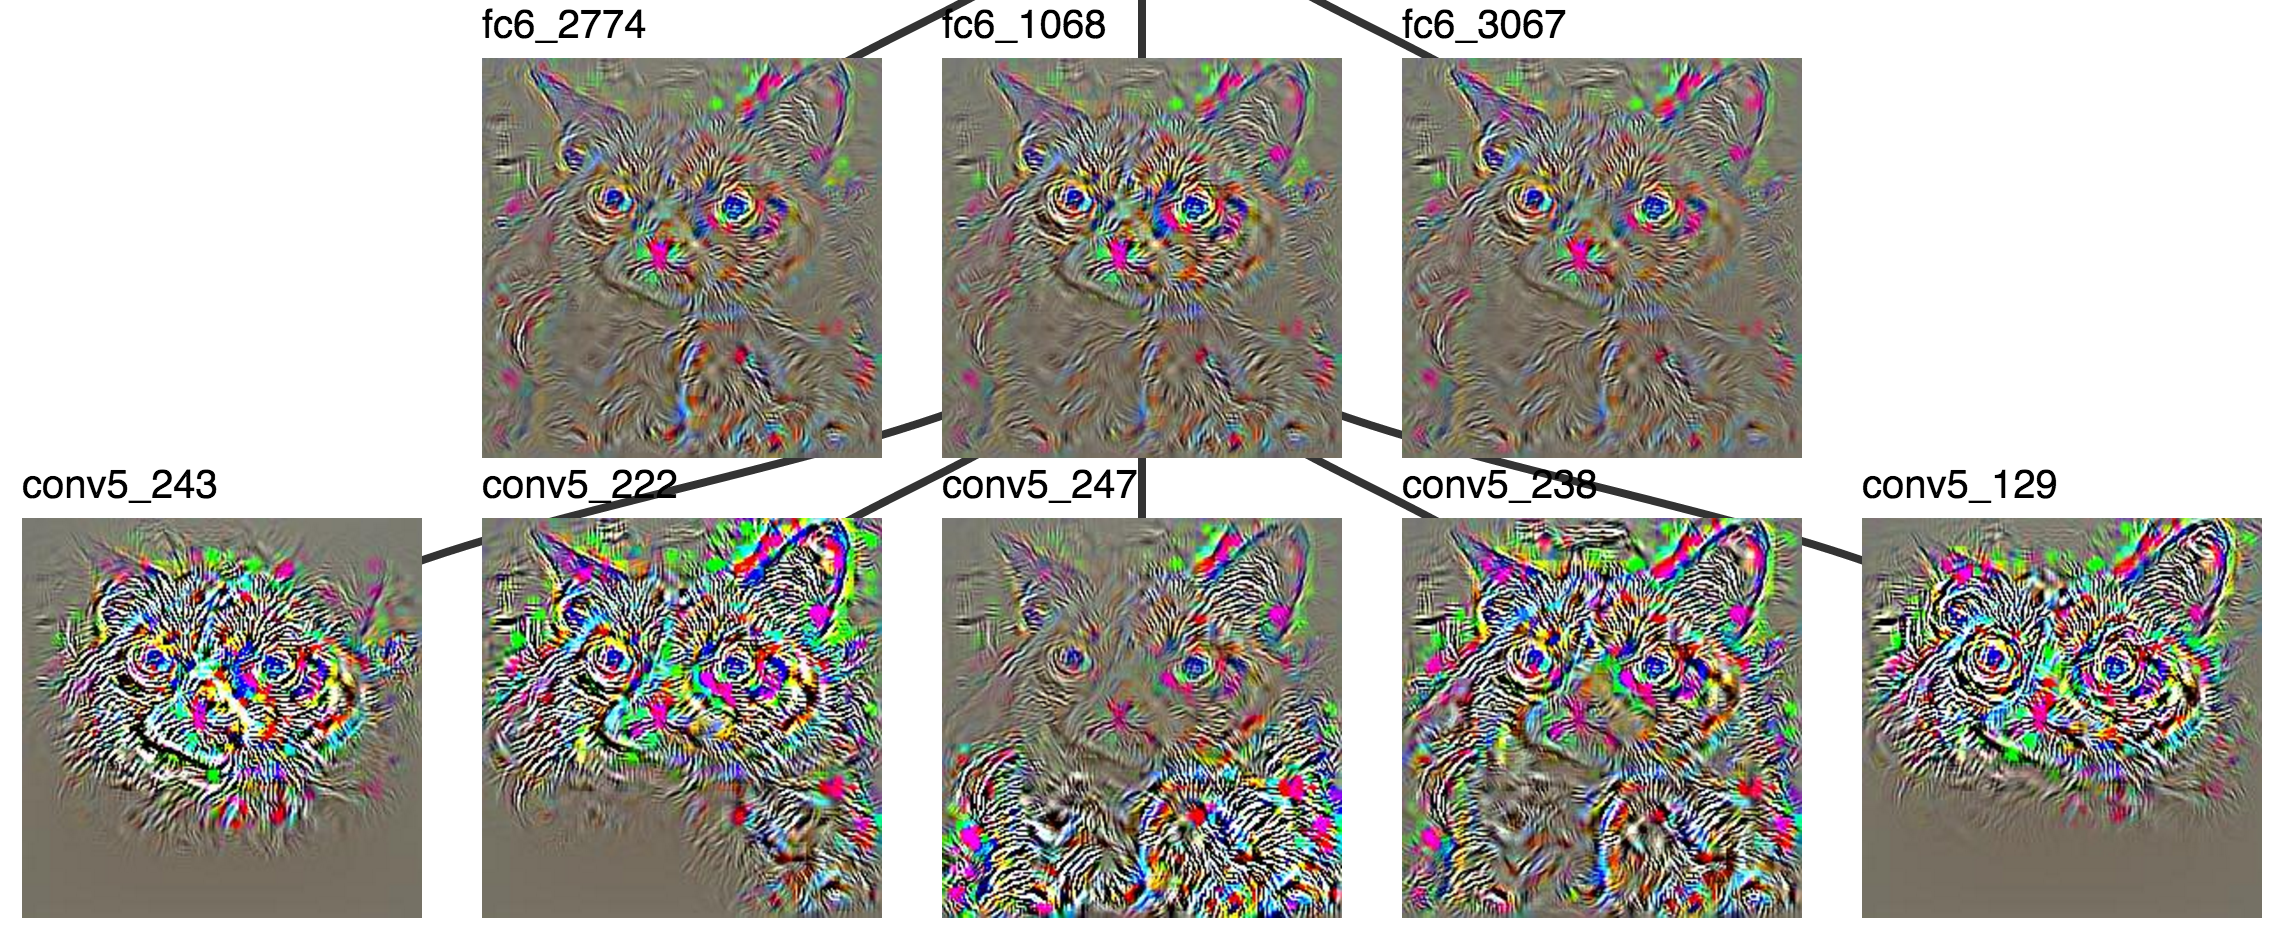
\includegraphics[width=0.5\textwidth]{Images/cat-features.png}
\caption{Cat edges recognized by individual CNN layers\protect\footnotemark}
\end{figure}


\footnotetext{Example detected egdes image from \url{https://en.wikipedia.org/wiki/Sobel_operator}}


\subsection{Convolution operation on volume}

Black and white images contain only single color channel, but in color images there are more. E.g. color RGB Image contains 3 channels (Red, Green, Blue). In that case each filter need to have 3 "sub filters", one for each channel. We apply convolution operation to each channel and then sum up the result (See Figure 6).  
\newline

\begin{figure}[ht]
\centering
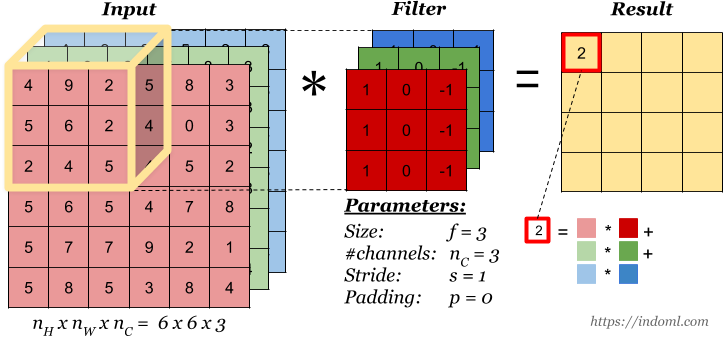
\includegraphics[width=0.5\textwidth]{Images/convolution-operation-on-volume.png}
\caption{Convolution on volume example [11]}
\end{figure}

\subsection{Multiple filters}

To detect multiple types of features in previous layer we should use multiple filters. E.g. one filter will detect vertical edges and one will detect horizontal (See Figure 7).


\begin{figure}[ht]
\centering
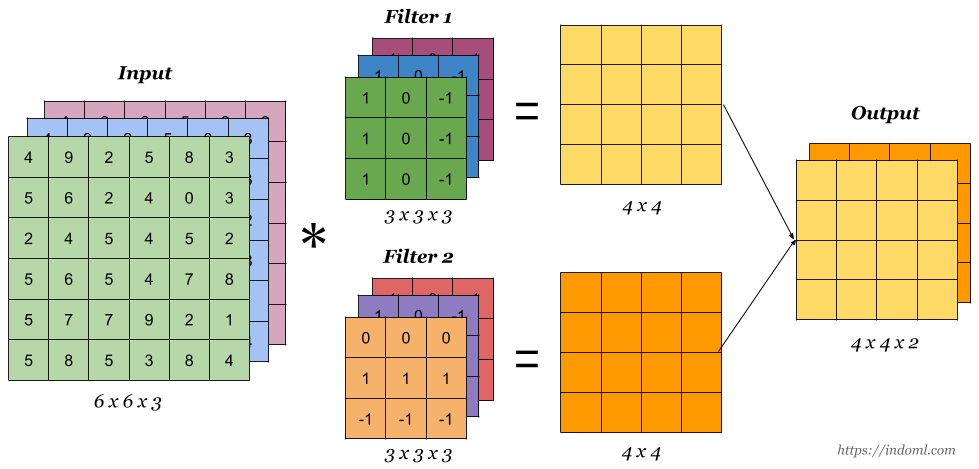
\includegraphics[width=0.5\textwidth]{Images/convolution-with-multiple-filters.png}
\caption{Convolution with multiple filters example[11]}
\end{figure}


\subsection{Padding}

To avoid underrepresentation of edge pixels it is worth to add one layer of extra pixels around original image (See Figure 8).


\begin{figure}
\centering
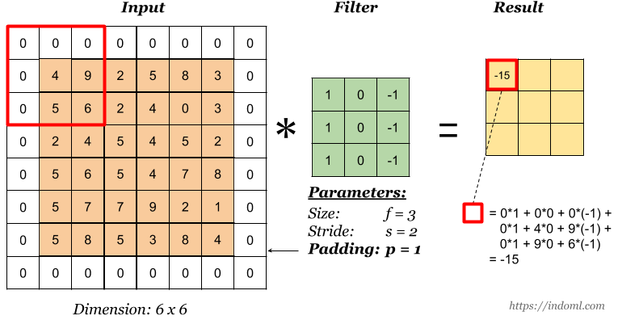
\includegraphics[width=0.5\textwidth]{Images/padding.png}
\caption{Example of 1 pixel padding [11]}
\end{figure}

\subsection{Stride}

Stride determines the number of cells that the filter moves in the input to calculate cell in output (See Figure 9).

\begin{figure}
\centering
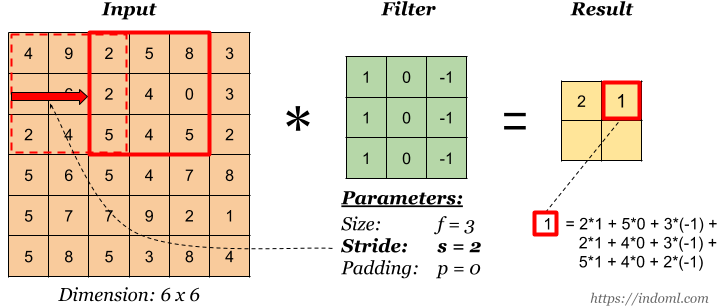
\includegraphics[width=0.5\textwidth]{Images/stride.png}
\caption{Example output for stride equal 2[11]}
\end{figure}

\subsection{Pooling layer}

Another type of layer used in CNNs is Pooling Layer. There are two types of Pooling Layers: Avg. Pooling and Max Pooling.  Pooling layers significantly reduce size of an image. The intuition behind pooling is \textit{take most important information} for Max Pooling and \textit{take average of all information} for Avg Pooling. (See Figure 10).

\begin{figure}
\centering
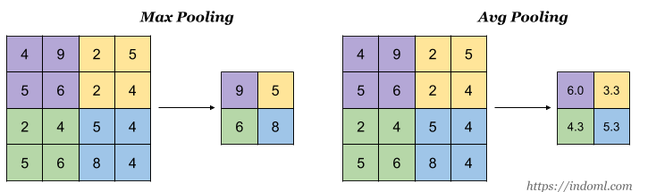
\includegraphics[width=0.5\textwidth]{Images/pooling-layer.png}
\caption{Outputs after pooling operations [11]}
\end{figure}


